\documentclass[tikz,border=5pt]{standalone}
\usepackage{amsmath,amssymb}
\begin{document}
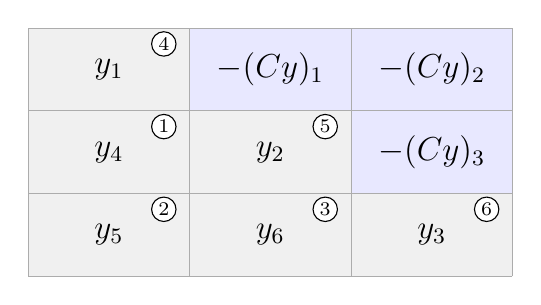
\begin{tikzpicture}[x=2.05cm,y=1.05cm,font=\large]
\fill[gray!12] (0,0) rectangle (3,-3);
\foreach \x/\y in {1/0,2/0,2/-1}{\fill[blue!9] (\x,\y) rectangle +(1,-1);}
\draw[gray!65] (0,0) grid[step=1] (3,-3);
\node at (.5,-.5) {$y_1$}; \node at (1.5,-1.5) {$y_2$}; \node at (2.5,-2.5) {$y_3$};
\node at (.5,-1.5) {$y_4$}; \node at (.5,-2.5) {$y_5$}; \node at (1.5,-2.5) {$y_6$};
\node at (1.5,-.5) {$-(Cy)_1$}; \node at (2.5,-.5) {$-(Cy)_2$}; \node at (2.5,-1.5) {$-(Cy)_3$};
\foreach \x/\y/\v in {.84/-.19/4,1.84/-1.19/5,2.84/-2.19/6,.84/-1.19/1,.84/-2.19/2,1.84/-2.19/3}
 {\node[draw,circle,inner sep=1pt,font=\scriptsize,fill=white] at (\x,\y) {\v};}
\end{tikzpicture}
\end{document}
